\documentclass{article}
\usepackage[T1]{fontenc}
\usepackage{lmodern}
\usepackage{graphicx}
\usepackage{amsmath,amssymb}
\usepackage[a4paper,margin=2cm]{geometry}
\usepackage[absolute,overlay]{textpos}
\setlength{\TPHorizModule}{1mm}
\setlength{\TPVertModule}{1mm}
\usepackage[indonesian]{babel}
\usepackage{hyperref}
\setlength{\emergencystretch}{2em}
% unit: Halaman 52

\begin{document}

% === Halaman 52 (llm) ===

\vspace{11.88mm}

\begin{itemize}
    \item Pada Contoh 2, 
    \begin{itemize}
        \item kunci = \texttt{abcdef}
        \item panjang kunci = 6
        \item jarak antara dua \texttt{crypto} yang berulang = 16
        \item 16 bukan kelipatan 6
    \end{itemize}
    $\therefore$ \texttt{crypto} tidak dienkripsi menjadi kriptogram yang sama
    
    \vspace{10mm}
    
    \item Goal metode Kasiski: mencari dua atau lebih kriptogram yang berulang untuk menentukan panjang kunci.
\end{itemize}

% deskripsi: Ilustrasi proses enkripsi Vigenere dengan teks plaintext, kunci, dan cipherteks, menunjukkan jarak antara kata 'crypto' yang berulang adalah 16 karakter.
% bbox normalisasi: [0.0600, 0.1080, 0.9400, 0.9120]
\begin{textblock*}{184.80mm}(12.60mm,32.08mm)
\noindent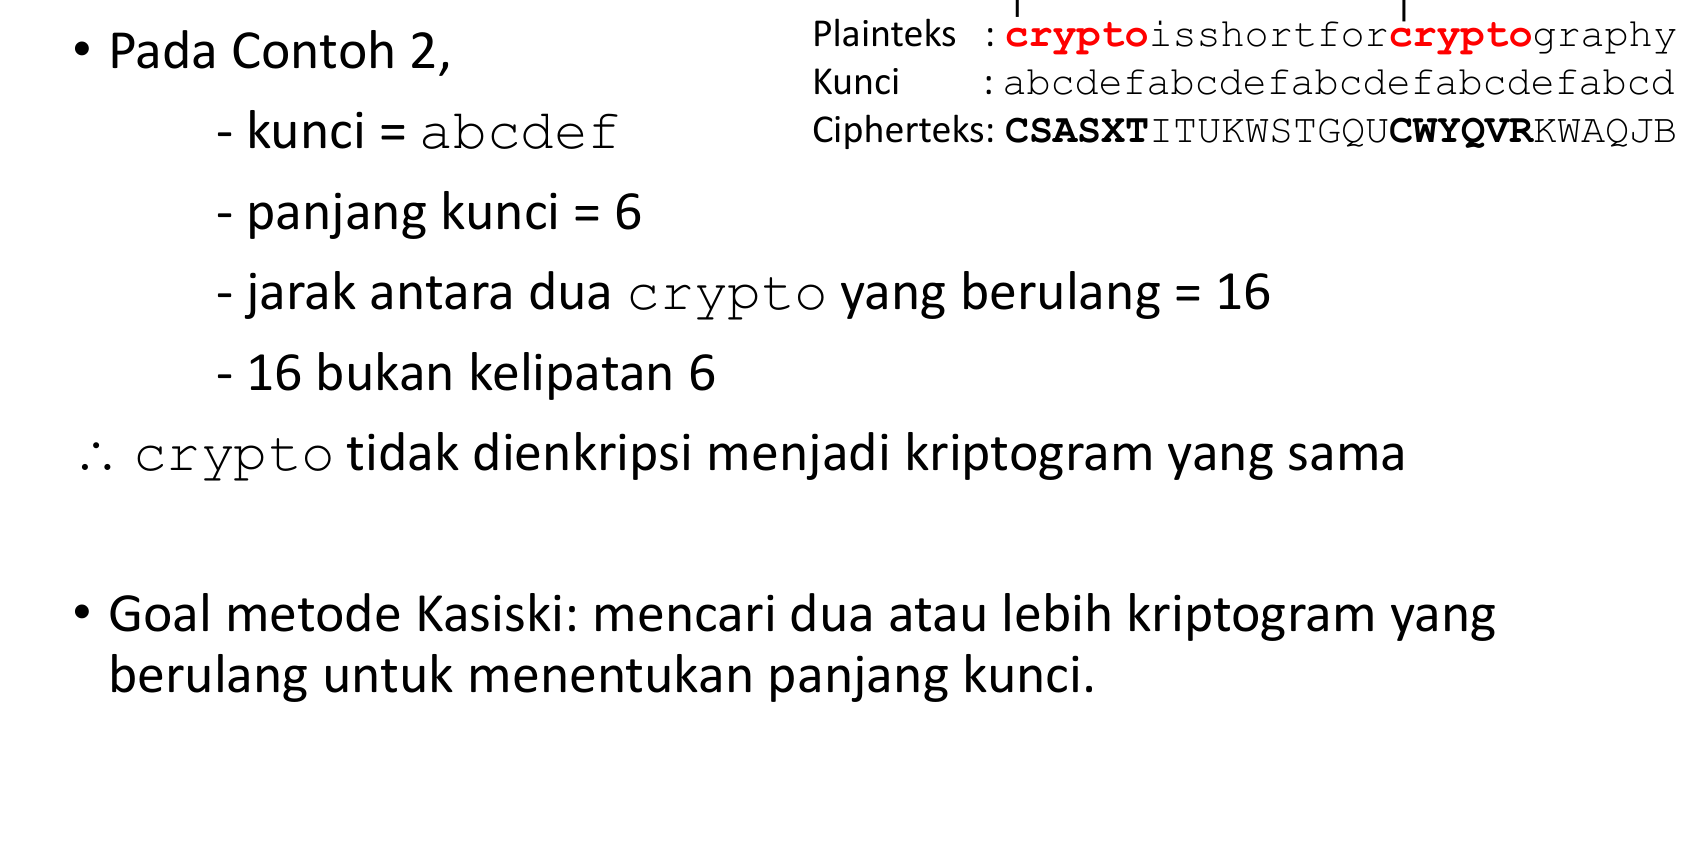
\includegraphics[width=184.80mm,height=238.79mm]{../../images/llm/page_052_img_01.png}%
\end{textblock*}

% deskripsi: Contoh perhitungan jarak antara dua kata 'crypto' yang berulang dalam plaintext yang diberi label angka 16.
% bbox normalisasi: [0.4800, 0.2000, 0.9400, 0.2400]
\begin{textblock*}{96.60mm}(100.80mm,59.40mm)
\noindent
\includegraphics[width=96.60mm,height=11.88mm]{../../images/llm/page_052_img_02.png}%
\end{textblock*}

% bbox perkiraan otomatis: Ilustrasi proses enkripsi Vigenere dengan teks plaintext, kunci, dan cipherteks, menunjukkan jarak antara kata 'crypto' yang berulang adalah 16 karakter.

\end{document}
